\documentclass[10pt,xcolor=svgnames]{beamer} %Beamer


\usepackage{palatino} %font type
\usepackage{xcolor}
\usepackage[font={tiny}]{caption}
\usefonttheme{metropolis} %Type of slides
\usefonttheme[onlymath]{serif} %font type Mathematical expressions
\usetheme[progressbar=frametitle,titleformat frame=smallcaps,numbering=counter]{metropolis} %This adds a bar at the beginning of each section.
\useoutertheme[subsection=false]{miniframes} %Circles in the top of each frame, showing the slide of each section you are at

\usepackage{appendixnumberbeamer} %enumerate each slide without counting the appendix

\definecolor{SysBlue}{RGB}{238,162,100}
\definecolor{Progress}{RGB}{56,60,92}
\definecolor{Header}{RGB}{0,0,0}
\definecolor{SlideTitle}{RGB}{213,213,213}
\definecolor{ToC}{RGB}{51,58,66}

\setbeamercolor{progress bar}{fg=SysBlue} %These are the colours of the progress bar. Notice that the names used are the svgnames
\setbeamercolor{title separator}{fg=SysBlue} %This is the line colour in the title slide
\setbeamercolor{structure}{fg=black} %Colour of the text of structure, numbers, items, blah. Not the big text.
\setbeamercolor{normal text}{fg=black!87} %Colour of normal text
\setbeamercolor{alerted text}{fg=DarkRed!60!Gainsboro} %Color of the alert box
\setbeamercolor{example text}{fg=ToC} %Colour of the Example block text
\setbeamercolor{background canvas}{bg=white}
\setbeamercolor{item}{fg=black}

\setbeamercolor{palette primary}{bg=SlideTitle, fg=ToC} %These are the colours of the background. Being this the main combination and so one. 
\setbeamercolor{palette secondary}{bg=ToC, fg=white}
\setbeamercolor{palette tertiary}{bg=ToC, fg=white}
\setbeamercolor{section in toc}{fg=ToC} %Color of the text in the table of contents (toc)

\setbeamertemplate{blocks}[rounded][shadow=true]


%These next packages are the useful for Physics in general, you can add the extras here. 
\usepackage{amsmath,amssymb}
\usepackage{slashed}
\usepackage{cite}
\usepackage{relsize}
\usepackage{caption}
\usepackage{subcaption}
\usepackage{multicol}
\usepackage{booktabs}
\usepackage[scale=2]{ccicons}
\usepackage{pgfplots}
\usepgfplotslibrary{dateplot}
\usepackage{geometry}
\usepackage{xspace}

\newcommand{\themename}{\textbf{\textsc{bluetemp}\xspace}}%metropolis}}\xspace}

\title{Pachira Fund}
\author[Name]{Ian Moore, PhD \inst{$\dagger$}}%With inst, you can change the institution they belong
\subtitle{Can Money Grow on Trees?}

\institute[shortinst]{\inst{$\dagger$} Tokenomics Researcher / Engineer @ Syslabs (email: imoore@syscoin.org) }

\date{November 13, 2023} %Here you can change the date
\titlegraphic{\vspace{-0.5cm}\hfill
\includegraphics[scale=0.23]{logo.png}} %You can modify the location of the logo by changing the command \vspace{}. 

\begin{document}
{
\setbeamercolor{background canvas}{bg=white, fg=black}
\setbeamercolor{normal text}{fg=black}
\maketitle
}%This is the colour of the first slide. bg= background and fg=foreground

\metroset{titleformat frame=smallcaps} %This changes the titles for small caps

\begin{frame}{Outline}
  \setbeamertemplate{section in toc}[sections numbered] %This is numbering the sections
  \tableofcontents[hideallsubsections] %You can comment this line if you want to show the subsections in the table of contents
\end{frame}

\section{Introduction}



\begin{frame}{Objectives}

\metroset{block=fill}
\begin{exampleblock}{\textsc{Define our problem}}
\begin{itemize}
  \item Stagnant Pool Problem
  \item Implicitly addressed by Uniswap v3
\end{itemize}  
\end{exampleblock}

\begin{exampleblock}{\textsc{Present our Solution}}
\begin{itemize}
  \item Liquidity Trees
  \item Simulation Results
\end{itemize}
\end{exampleblock}

\begin{exampleblock}{\textsc{Objective Revisted}}
\begin{itemize}
  \item Can Money Grow on Trees?
\end{itemize}
\end{exampleblock}

\end{frame}


\section{What are we Solving?}

\begin{frame}{Stagnant Pool Problem} 

\metroset{block=fill}
\begin{exampleblock}{\textsc{Lay Definition:}}
\begin{itemize}
  \item How do we increase $\Delta V$ on liquidity over some time interval $t$?
\end{itemize}
\end{exampleblock}

\begin{exampleblock}{\textsc{Uniswap v3 has implicitly addressed this problem:}}
\begin{itemize}
  \item Increasing the depth of order book (virtually)
  \item Makes large trades more efficient
  \item Hence increasing the \textit{possibility} of more $\Delta V$
  \item However, does nothing to induce more trading volume
\end{itemize}
\end{exampleblock}


\end{frame}


\begin{frame}{Uniswap v3} 

\begin{figure}[h!]
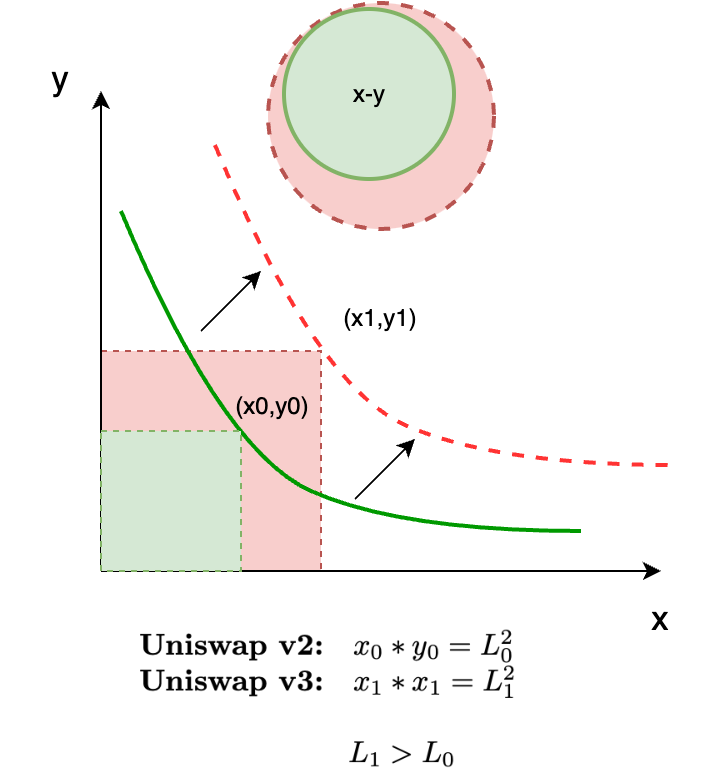
\includegraphics[width=2.3in]{img/uniswap_v3.png}
\caption{Graphical illustration on how depth is virtually increased using Uniswap v3} 
\label{fig:uniswap_v3}
\end{figure}

\end{frame}

\begin{frame}{Indexing Problem: Posed} 

\metroset{block=fill}
\begin{exampleblock}{\textsc{CPT Indexing Problem}}
\begin{itemize}
  \item Given a position $\Delta L$, what is the indexed value in only one of the two pairing assets (x,y)
\end{itemize}
\end{exampleblock}

\begin{figure}[h!]
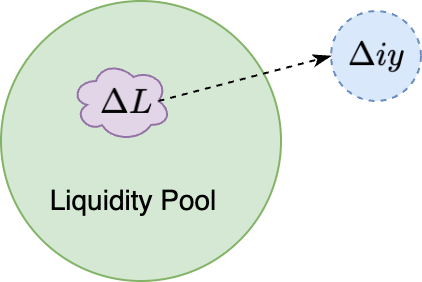
\includegraphics[width=2.3in]{img/indexed_tkn_lrg.png}
\label{fig:uniswap_v3}
\end{figure}



\end{frame}


\begin{frame}{Indexing Problem: Solution} 

This system describes the mathematical operations that are effectively being done in the contract code when performing an \textit{efficient} two-step withdrawal (ie, withdrawal both assets + swap one for the remaining) operation: 

\begin{align}
\Delta x &=\frac{\Delta L x}{L}\\
\Delta y &=\frac{\Delta L y}{L}\\
\Delta y_{(i)} &= \Delta y + \frac{\gamma \Delta x (y - \Delta y)}{(x - \Delta x) + \gamma \Delta x}
\end{align}

\end{frame}


\begin{frame}{Let's Include a new Dimension ...} 
 
\begin{figure}[h!]
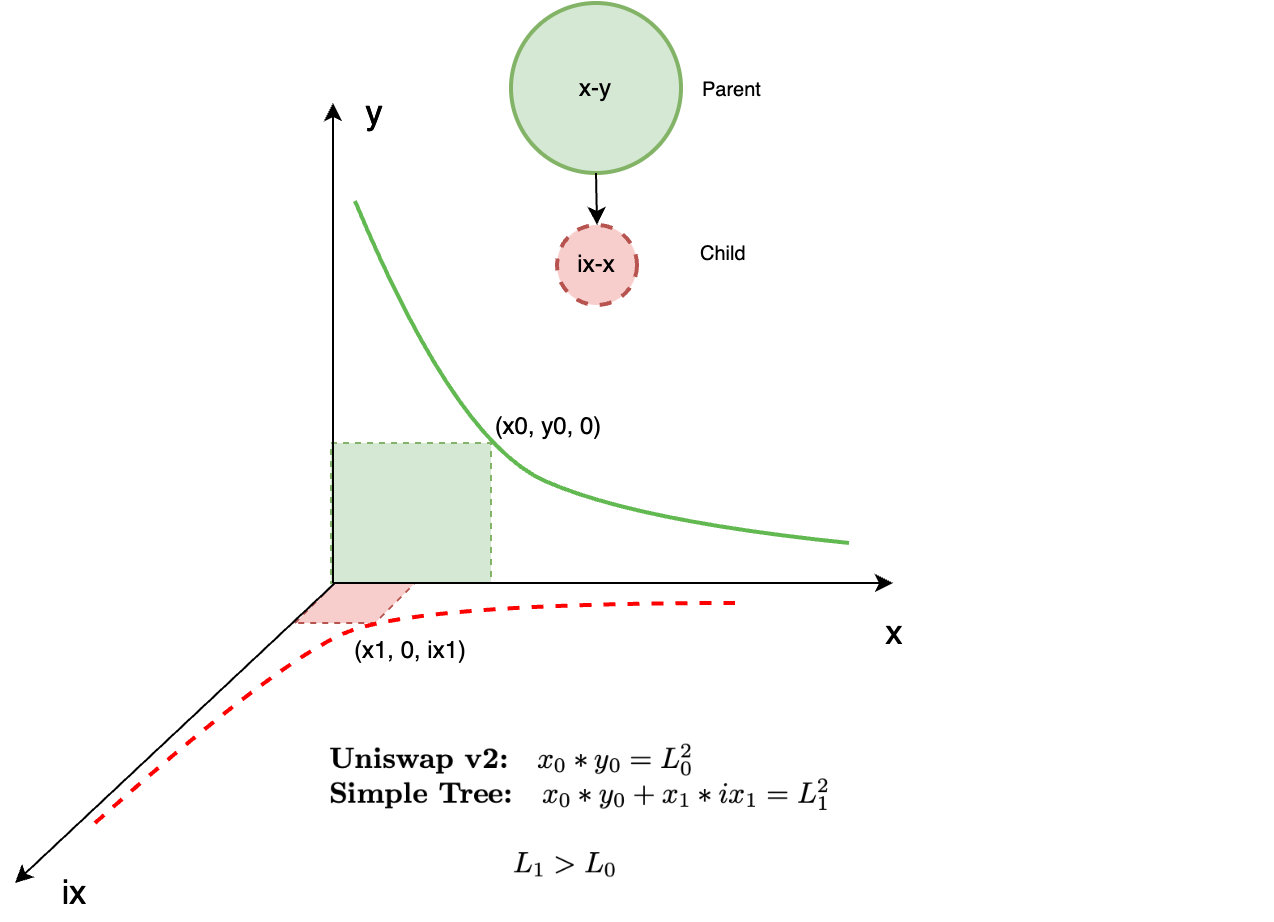
\includegraphics[width=3in]{img/simple_tree.png}
\caption{Simple Tree} 
\label{fig:simple_tree}
\end{figure}

\end{frame}

\begin{frame}{New Dimension Cont'} 

\begin{figure}[h!]
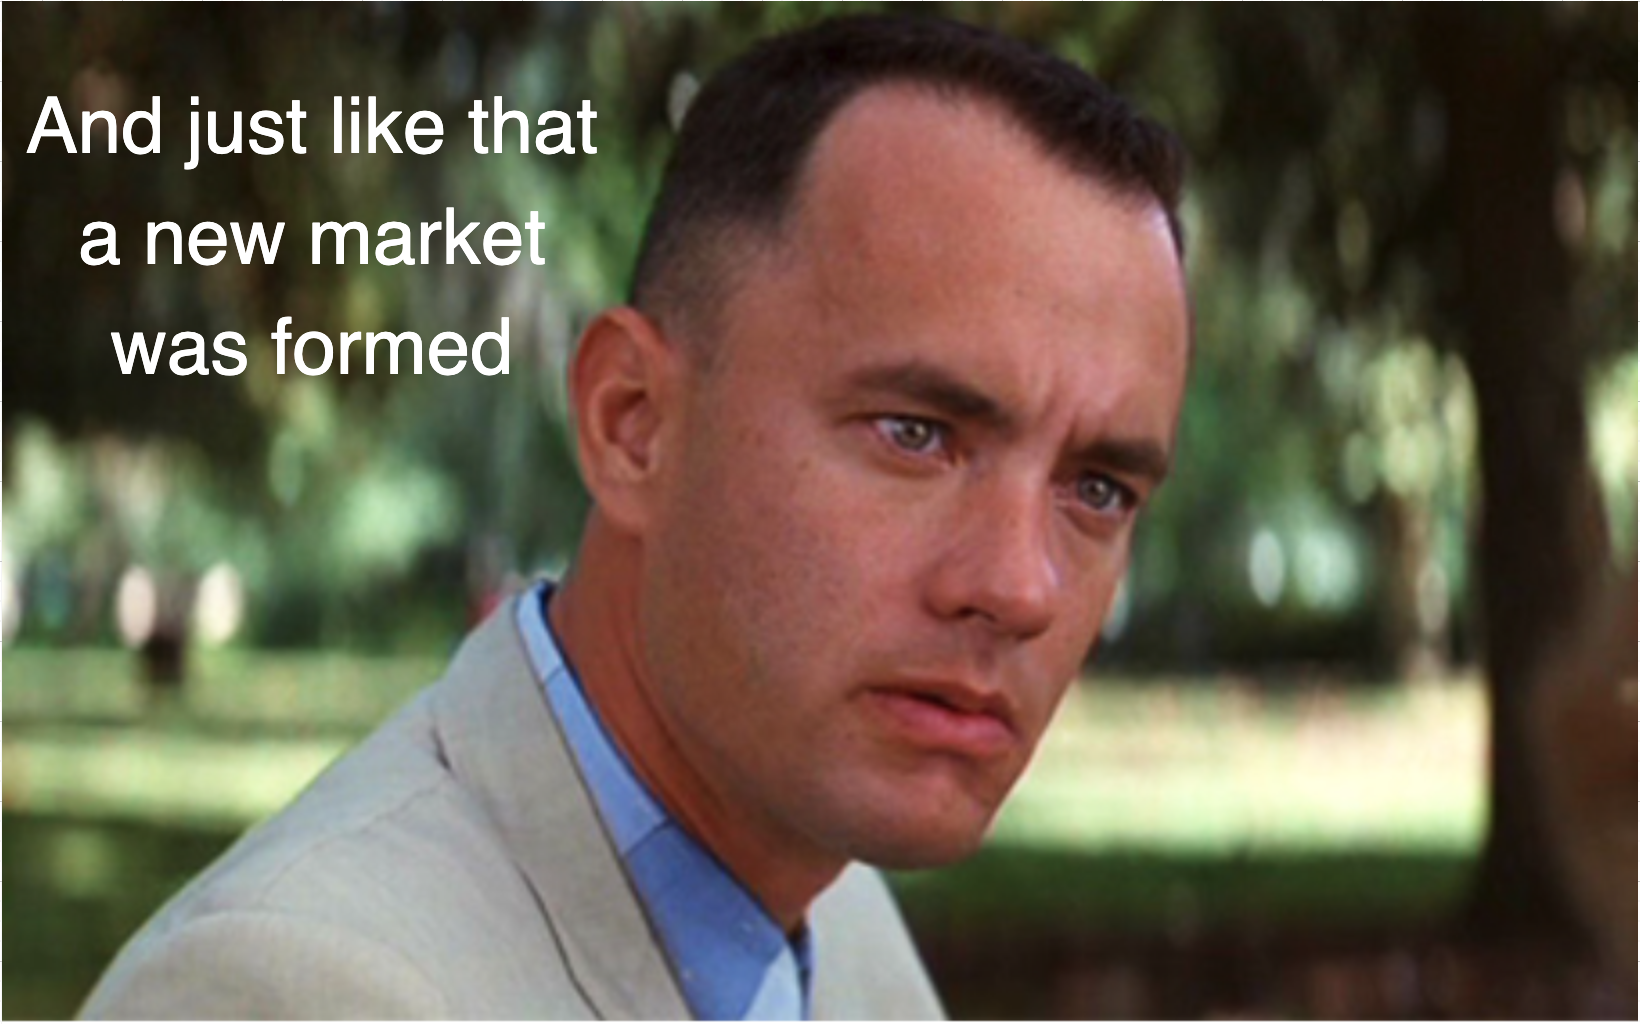
\includegraphics[width=3in]{img/gump.png}
\label{fig:gump}
\end{figure}

\end{frame}

\begin{frame}{How does this Work?} 

\begin{figure}[h!]
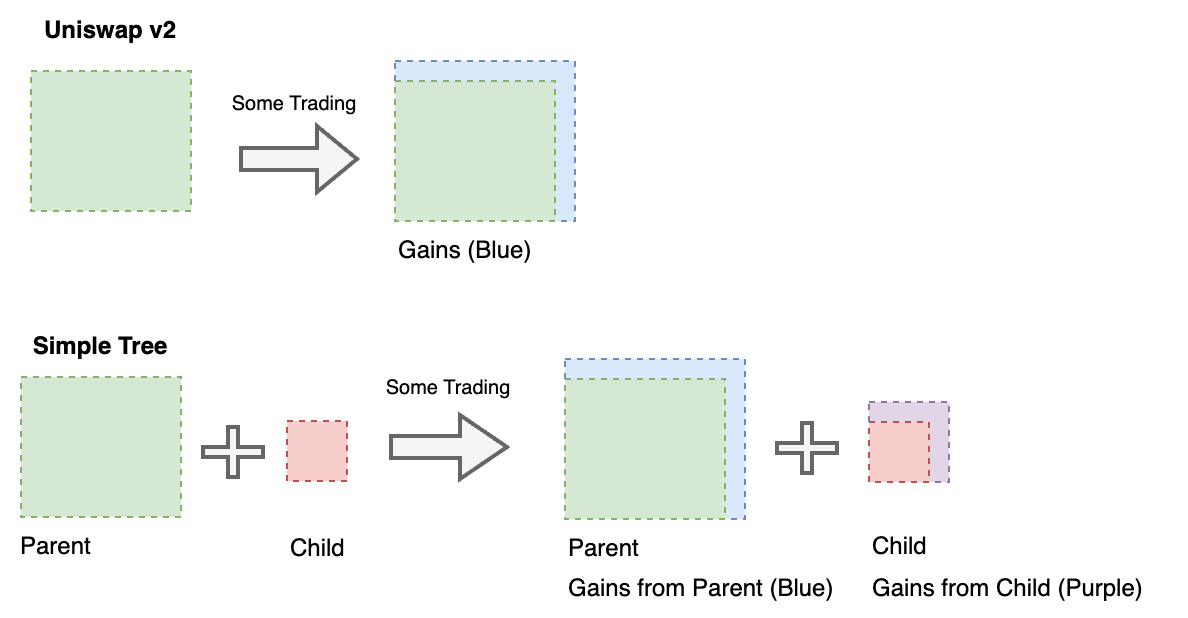
\includegraphics[width=3in]{img/compare.png}
\caption{Boxes represent liquidity under CPT curve; creating a new market out of indexed liquidity indexed liquidity is a way to address the stagnant pool problem; in short we've leveraged some of the green, got red and made some extra purple} 
\label{fig:compare}
\end{figure}

\end{frame}



\section{Liquidity Trees}

\begin{frame}{Full Tree} 

\begin{figure}[h!]
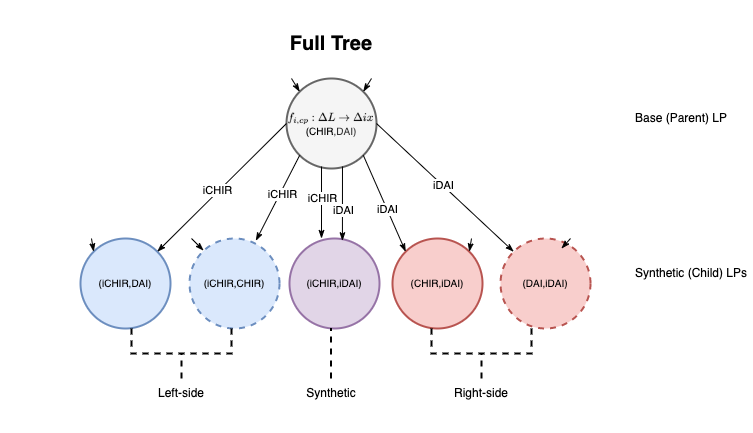
\includegraphics[width=3in]{img/full_tree.png}
\caption{Full CPT liquidity tree represented as a computational tree structure comprised of left-sided, right-sided and synthetic pools } 
\label{fig:full_tree}
\end{figure}

\end{frame}

\begin{frame}{Sub Trees} 

\begin{figure}[h!]
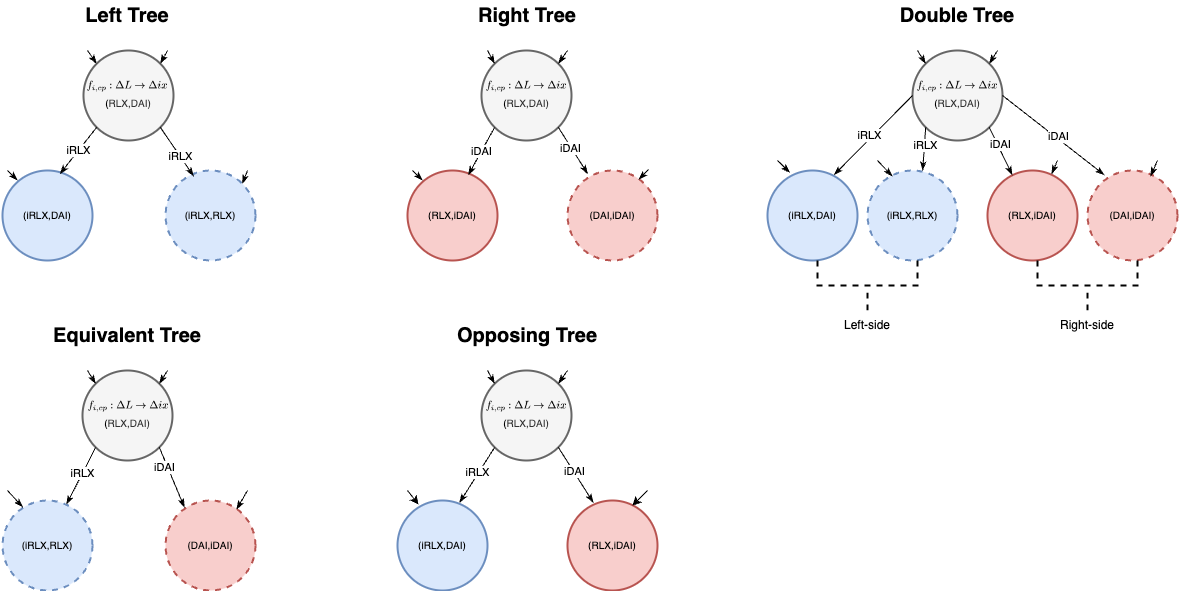
\includegraphics[width=3in]{img/sub_trees.png}
\caption{Sub-trees comprised of: (TOP LEFT) left tree; (TOP CENTER) right tree; (TOP RIGHT) double tree; (BOTTOM LEFT) equivalent tree; (BOTTOM CENTER) opposing Tree} 
\label{fig:sub_trees}
\end{figure}

\end{frame}


\section{Simulation Results}

\begin{frame}{Left Tree}

\begin{figure}[h!]
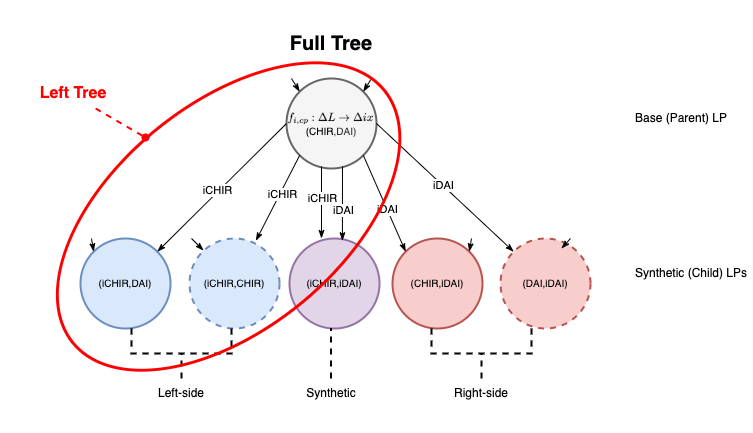
\includegraphics[width=3in]{img/left_tree.png}
\caption{Left Tree} 
\label{fig:left_tree}
\end{figure}

\end{frame}


\begin{frame}{Left Tree: Simulated Price / Revenue (1)}

\begin{figure}[h!]
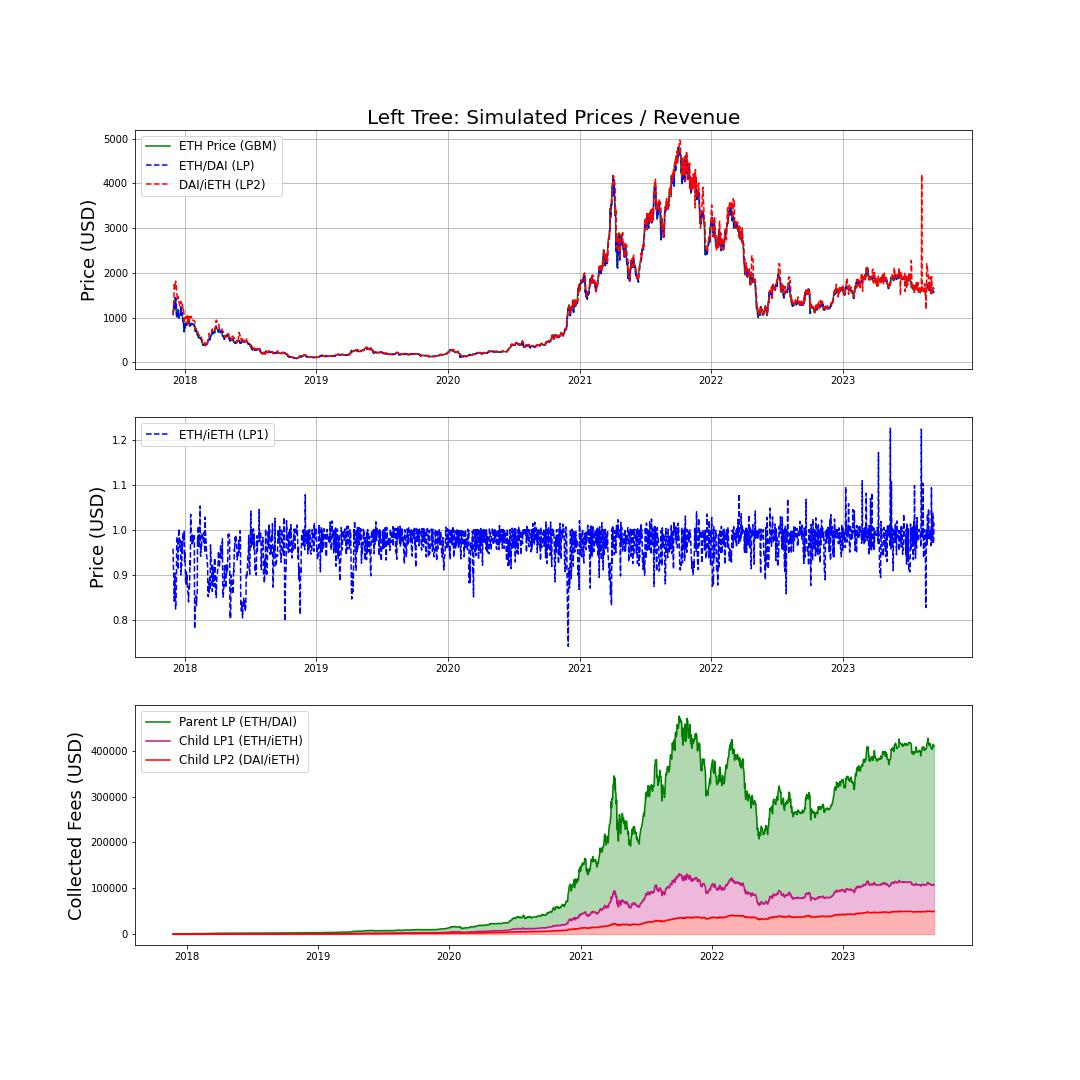
\includegraphics[width=3in]{img/simulation.jpg}
\label{fig:simulation}
\end{figure}

\end{frame}


\begin{frame}{Left Tree: Simulated Price / Revenue (2)}


\begin{table}[h]
\tiny
\centering
\begin{tabular}{ |l|c|c|c| } 
\hline
 \textbf{Metric} & \multicolumn{3}{|c|}{\textbf{Totals}}\\
\hline 
 Revenue (LP) / LP Liquidity & \multicolumn{3}{|c|}{19.4\% }\\
 Revenue (LP+LP1+LP2) / LP Liquidity & \multicolumn{3}{|c|}{26.3\% }\\
 Revenue Boost (Indexed Liquidity)  & \multicolumn{3}{|c|}{35.61\%}\\ 
 Percentage Indexed & \multicolumn{3}{|c|}{7.51\%}\\ 
 \hline
\hline
	& \multicolumn{3}{|c|}{\textbf{Sub-totals}} \\
  & \textbf{LP (ETH-DAI)} & \textbf{LP1 (iETH-ETH)} & \textbf{LP2 (iETH-DAI)} \\
\hline
Liquidity  & \$1,559,145 & \$71,961 & \$162,118\\
Revenue  & \$302,140 & \$57,927 & \$49,673\\
Revenue / Liquidity  & 19.4\% & 80.5\% & 30.64\%\\ 
\hline
\end{tabular}
\caption{Metrics harvested from Left-tree simulation using ETH \& DAI (Jan 2018 to Oct 2023)}
\label{table:simulator_components}
\end{table}

\end{frame}



\section{Revist our Objective}

\begin{frame}{In Summary}


\metroset{block=fill}
\begin{exampleblock}{\textsc{Stagnant Pool Problem}}
\begin{itemize}
  \item Shown how stagnant pool problem can be addressed
\end{itemize}
\end{exampleblock}

\begin{exampleblock}{\textsc{Liquidity Trees: A new DeFi Primitive}}
\begin{itemize}
  \item New DeFi Primitive, which we call Liquidity Trees 
  \item Utilizes fully collateralized liquidity, and can be represented as undirected graphs or algebraically in $\mathbb{R}^n$
\end{itemize}
\end{exampleblock}

\begin{exampleblock}{\textsc{Pachira Token Launch}}
\begin{itemize}
  \item Combining thes Liquidity Trees with a Governance system for Pachira Fund token launch
\end{itemize}
\end{exampleblock}



\end{frame}


\begin{frame}[standout]
  Thank you! 
\end{frame}

\begin{frame}{Appendix 1: Pachira Token Launch}
\begin{figure}[h!]
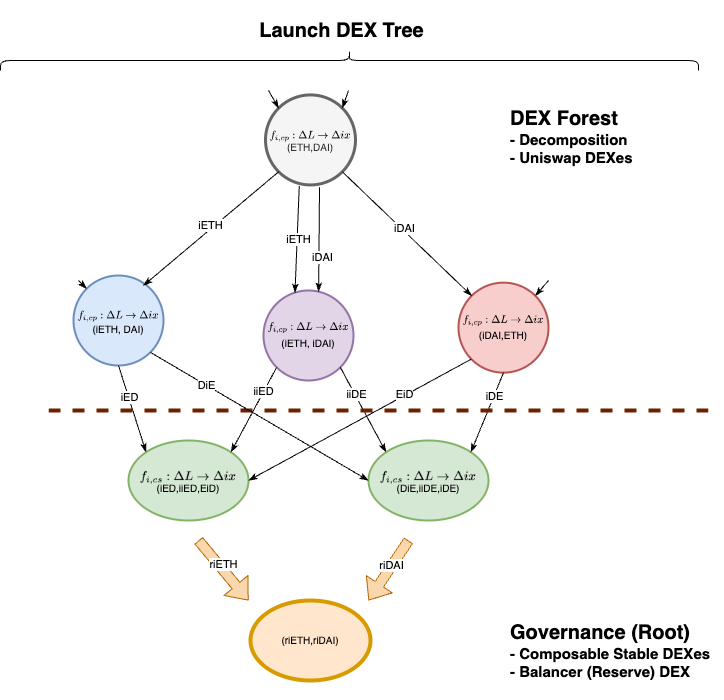
\includegraphics[width=3in]{img/dex_forest_single_tree.png}
\label{fig:dex_forest}
\end{figure}
\end{frame}

\begin{frame}{Appendix 2: Reserve Swap Prices}
\begin{figure}[h!]
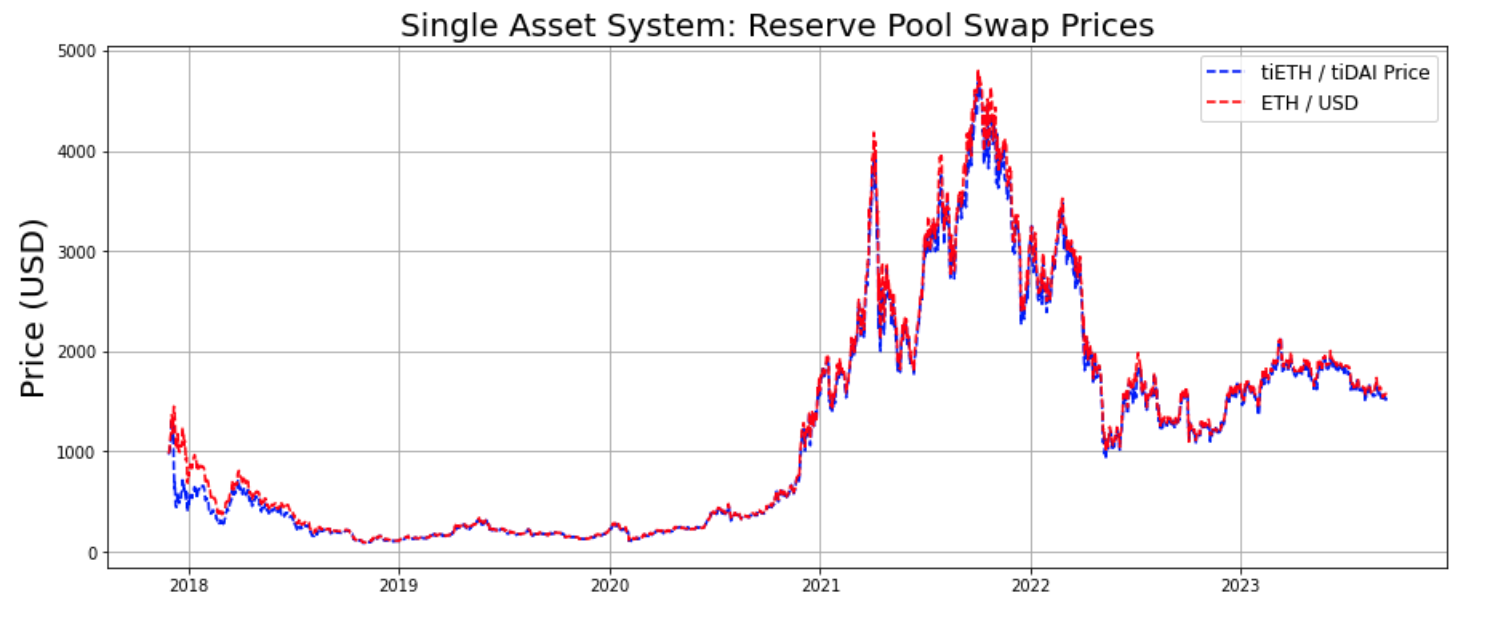
\includegraphics[width=3.5in]{img/single_swap_prices.png}
\label{fig:swap_prices}
\end{figure}
\end{frame}

\begin{frame}{Appendix 3: Pachira Token Launch}
\begin{figure}[h!]
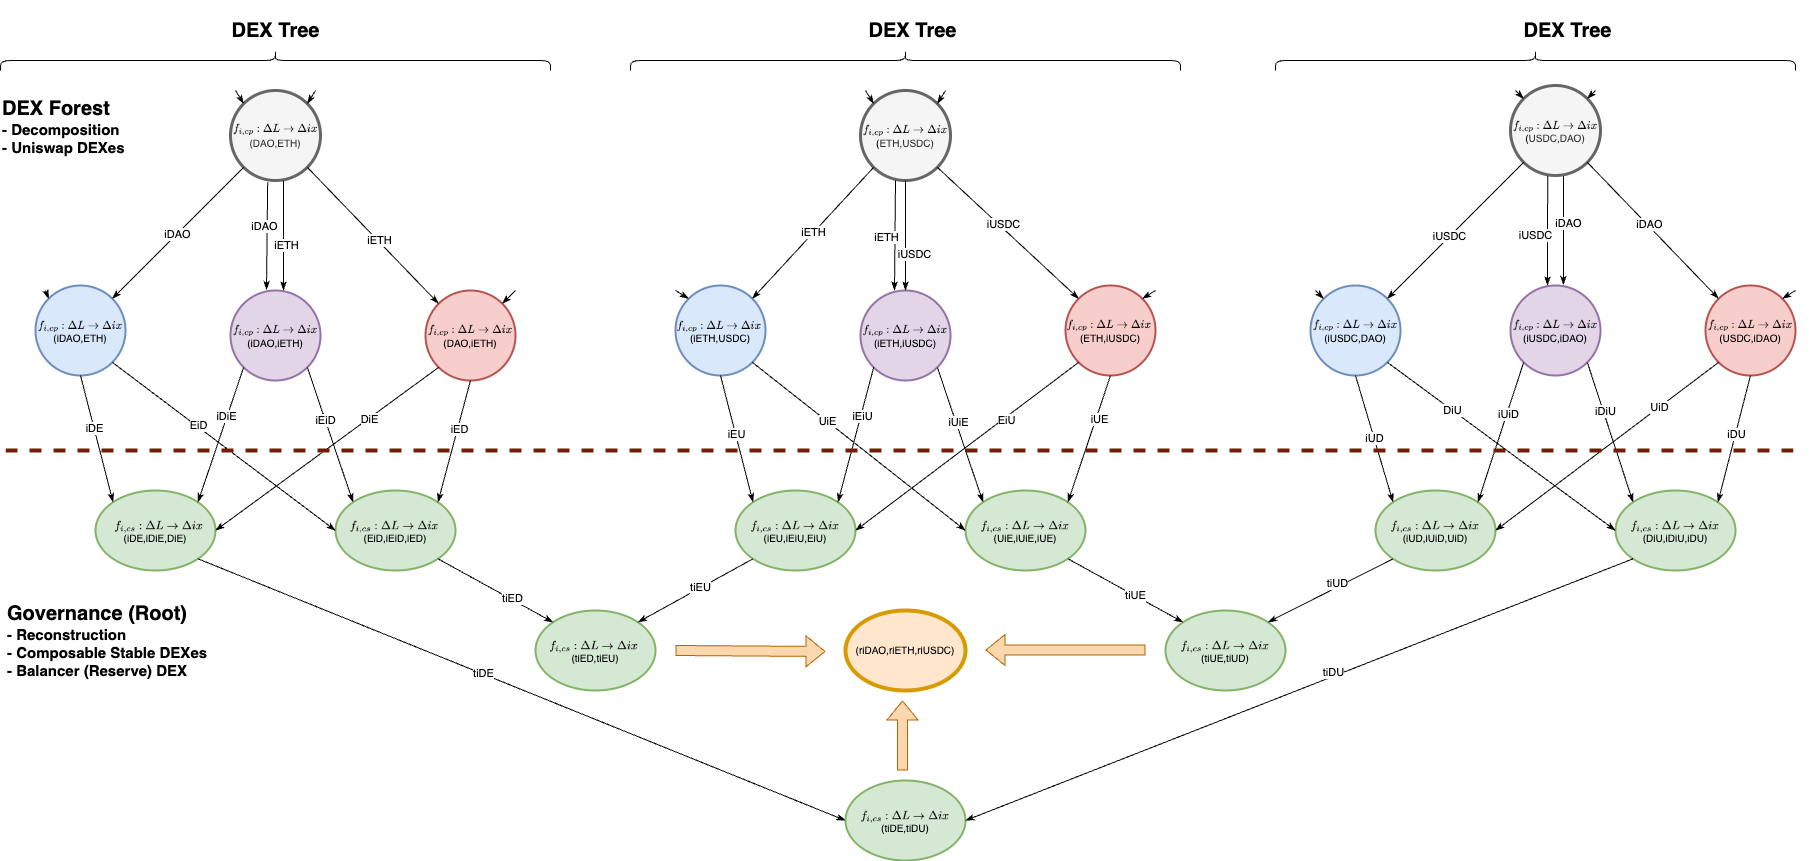
\includegraphics[width=4.2in]{img/dex_forest.png}
\label{fig:dex_forest}
\end{figure}
\end{frame}

\begin{frame}{Appendix 4: Reserve Swap Prices}
\begin{figure}[h!]
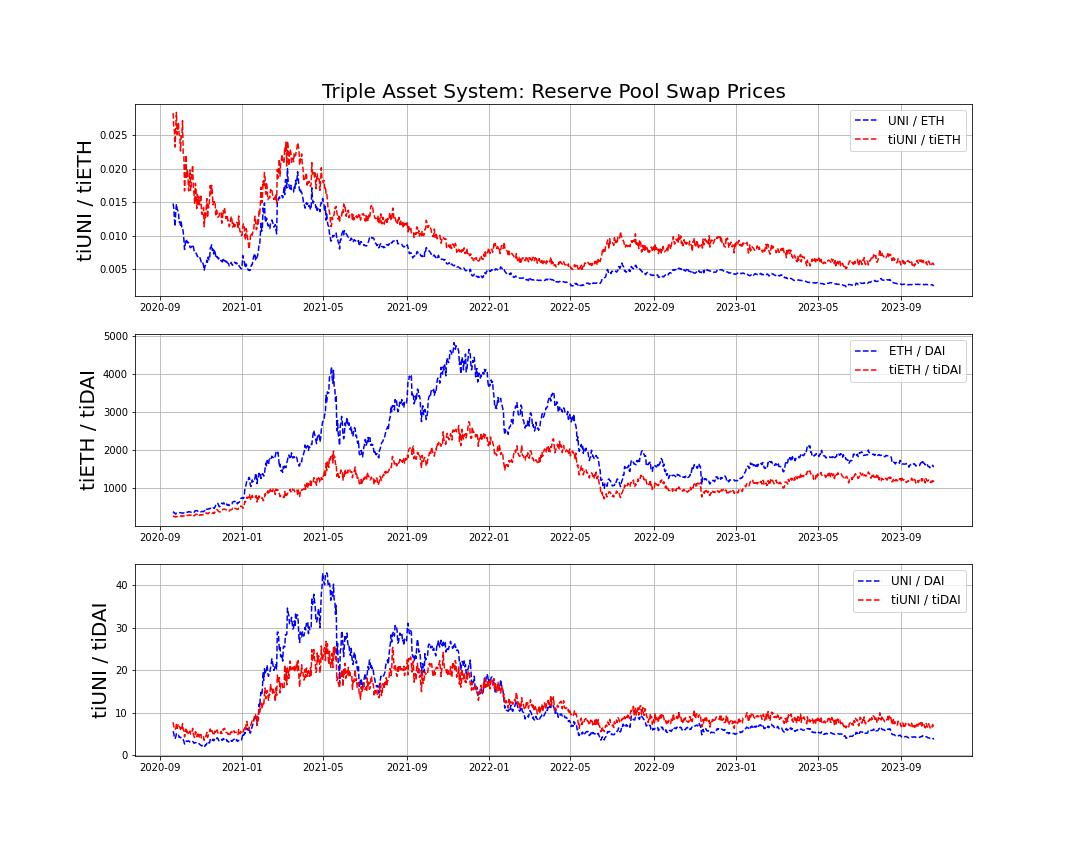
\includegraphics[width=3.5in]{img/swap_prices.jpg}
\label{fig:swap_prices}
\end{figure}
\end{frame}

\end{document}